\section{Capturing ADTs Structure} \label{sec:hrepcont}

\begin{figure*}[t]
  \centering
  \section{Extracting Structure} \label{sec:hrep}

In this work, we ...

\begin{code}
data HRep_Val  a = Mk_Val Int
data HRep_Add  a = Mk_Add a a
data HRep_Mul  a = Mk_Mul a a
\end{code}

For this purpose, we employ Haskell's type classes mechanism \tocite{}.
%
We define an evaluation type class $(\Downarrow)$ which specifies how to perform
a single transformation |step| from the higher-order representation back into a
concrete value of the target:

\begin{code}
class (rep down target) where
  step :: rep target -> target
\end{code}

Then, we can define the following overloaded instances of the |step| operation
for the canonical representations of data constructors simply by mapping each
lifted constructor back into its corresponding one.

\begin{code}
instance (HRep_Val down Exp) where
  step (Mk_Val n) = Val n

instance (HRep_Add down Exp) where
  step (Mk_Add x y) = Add x y

instance (HRep_Mul down Exp) where
  step (Mk_Mul x y) = Mul x y
\end{code}

With these individual representations, we can define a type combinator
$(\oplus)$ to compose two representations into a single one:

\begin{code}
data (f oplus g) a = L (f a) | R (g a)
\end{code}

Then, a composite representation can be transformed back into the concrete
target type by pattern matching on the data type variant and applying the |step|
tranformation to the inner representation:

\begin{code}
instance (f oplus g down Exp) where
  step (L f) = step f
  step (R g) = step g
\end{code}

Furthermore, we can define a type combinator ($\otimes$) to tag every
representation with an explicit generation frequency:

\begin{code}
data (f otimes n) a = Freq (f a)
\end{code}

This combinator is evaluated back to our target data type simply by piping the
result from the inner representation.
%
It does not change the evaluation semantics, as it is only considered at
generation time:

\begin{code}
instance (f otimes n down Exp) where
  step (Freq f) = step f
\end{code}

With the introduced combinators, we can easily create a type synonym |HRep_Exp|
to refer to the canonical representation of our original data type |Exp|,
tagging for instance the representation of the constuctor |Add| to be generated
in double the proportion of rest of the representations:

\begin{code}
type HRep_Exp  =       HRep_Val
               oplus'  HRep_Add  otimes 2
               oplus'  HRep_Mul
\end{code}



\begin{code}
data HRep_foo_1  a = Mk_foo_1 a a
data HRep_foo_2  a = Mk_foo_2 Int a
\end{code}

\begin{code}
instance (HRep_foo_1 down Exp) where
  step (Mk_foo_1 x y)
    = Add (Add x (Val 50)) (Add (Val 25) y)

instance (HRep_foo_2 down Exp) where
  step (Mk_foo_2 x y)
    = Mul (Val 50) (Mul (Val x) y)
\end{code}

\begin{code}
type HRep_foo  =       HRep_foo_1
               oplus'  HRep_foo_2
\end{code}


\begin{code}
data HRep_ten       a = Mk_ten
data HRep_square    a = Mk_square   a
data HRep_minus     a = Mk_minus    a a
\end{code}

\begin{code}
instance (HRep_ten down Exp) where
  step Mk_ten = ten

instance (HRep_square down Exp) where
  step (Mk_square x) = square x

instance (HRep_minus down Exp) where
  step (Mk_minus x y) = minus x y
\end{code}


\begin{code}
type HRep_M  =       HRep_ten
             oplus'  HRep_square
             oplus'  HRep_minus
\end{code}



\begin{code}
type Spec_Exp  =       HRep_Exp  otimes 4
               oplus'  HRep_foo  otimes 2
               oplus'  HRep_M
\end{code}

This previous definition can be interpreted graphically as it is shown in the
Figure \ref{fig:hrep}.
%
Curly arrows represent the structural information extracted using
meta-programming.

\begin{figure}[t]
  \centering
  \section{Extracting Structure} \label{sec:hrep}

In this work, we ...

\begin{code}
data HRep_Val  a = Mk_Val Int
data HRep_Add  a = Mk_Add a a
data HRep_Mul  a = Mk_Mul a a
\end{code}

For this purpose, we employ Haskell's type classes mechanism \tocite{}.
%
We define an evaluation type class $(\Downarrow)$ which specifies how to perform
a single transformation |step| from the higher-order representation back into a
concrete value of the target:

\begin{code}
class (rep down target) where
  step :: rep target -> target
\end{code}

Then, we can define the following overloaded instances of the |step| operation
for the canonical representations of data constructors simply by mapping each
lifted constructor back into its corresponding one.

\begin{code}
instance (HRep_Val down Exp) where
  step (Mk_Val n) = Val n

instance (HRep_Add down Exp) where
  step (Mk_Add x y) = Add x y

instance (HRep_Mul down Exp) where
  step (Mk_Mul x y) = Mul x y
\end{code}

With these individual representations, we can define a type combinator
$(\oplus)$ to compose two representations into a single one:

\begin{code}
data (f oplus g) a = L (f a) | R (g a)
\end{code}

Then, a composite representation can be transformed back into the concrete
target type by pattern matching on the data type variant and applying the |step|
tranformation to the inner representation:

\begin{code}
instance (f oplus g down Exp) where
  step (L f) = step f
  step (R g) = step g
\end{code}

Furthermore, we can define a type combinator ($\otimes$) to tag every
representation with an explicit generation frequency:

\begin{code}
data (f otimes n) a = Freq (f a)
\end{code}

This combinator is evaluated back to our target data type simply by piping the
result from the inner representation.
%
It does not change the evaluation semantics, as it is only considered at
generation time:

\begin{code}
instance (f otimes n down Exp) where
  step (Freq f) = step f
\end{code}

With the introduced combinators, we can easily create a type synonym |HRep_Exp|
to refer to the canonical representation of our original data type |Exp|,
tagging for instance the representation of the constuctor |Add| to be generated
in double the proportion of rest of the representations:

\begin{code}
type HRep_Exp  =       HRep_Val
               oplus'  HRep_Add  otimes 2
               oplus'  HRep_Mul
\end{code}



\begin{code}
data HRep_foo_1  a = Mk_foo_1 a a
data HRep_foo_2  a = Mk_foo_2 Int a
\end{code}

\begin{code}
instance (HRep_foo_1 down Exp) where
  step (Mk_foo_1 x y)
    = Add (Add x (Val 50)) (Add (Val 25) y)

instance (HRep_foo_2 down Exp) where
  step (Mk_foo_2 x y)
    = Mul (Val 50) (Mul (Val x) y)
\end{code}

\begin{code}
type HRep_foo  =       HRep_foo_1
               oplus'  HRep_foo_2
\end{code}


\begin{code}
data HRep_ten       a = Mk_ten
data HRep_square    a = Mk_square   a
data HRep_minus     a = Mk_minus    a a
\end{code}

\begin{code}
instance (HRep_ten down Exp) where
  step Mk_ten = ten

instance (HRep_square down Exp) where
  step (Mk_square x) = square x

instance (HRep_minus down Exp) where
  step (Mk_minus x y) = minus x y
\end{code}


\begin{code}
type HRep_M  =       HRep_ten
             oplus'  HRep_square
             oplus'  HRep_minus
\end{code}



\begin{code}
type Spec_Exp  =       HRep_Exp  otimes 4
               oplus'  HRep_foo  otimes 2
               oplus'  HRep_M
\end{code}

This previous definition can be interpreted graphically as it is shown in the
Figure \ref{fig:hrep}.
%
Curly arrows represent the structural information extracted using
meta-programming.

\begin{figure}[t]
  \centering
  \section{Extracting Structure} \label{sec:hrep}

In this work, we ...

\begin{code}
data HRep_Val  a = Mk_Val Int
data HRep_Add  a = Mk_Add a a
data HRep_Mul  a = Mk_Mul a a
\end{code}

For this purpose, we employ Haskell's type classes mechanism \tocite{}.
%
We define an evaluation type class $(\Downarrow)$ which specifies how to perform
a single transformation |step| from the higher-order representation back into a
concrete value of the target:

\begin{code}
class (rep down target) where
  step :: rep target -> target
\end{code}

Then, we can define the following overloaded instances of the |step| operation
for the canonical representations of data constructors simply by mapping each
lifted constructor back into its corresponding one.

\begin{code}
instance (HRep_Val down Exp) where
  step (Mk_Val n) = Val n

instance (HRep_Add down Exp) where
  step (Mk_Add x y) = Add x y

instance (HRep_Mul down Exp) where
  step (Mk_Mul x y) = Mul x y
\end{code}

With these individual representations, we can define a type combinator
$(\oplus)$ to compose two representations into a single one:

\begin{code}
data (f oplus g) a = L (f a) | R (g a)
\end{code}

Then, a composite representation can be transformed back into the concrete
target type by pattern matching on the data type variant and applying the |step|
tranformation to the inner representation:

\begin{code}
instance (f oplus g down Exp) where
  step (L f) = step f
  step (R g) = step g
\end{code}

Furthermore, we can define a type combinator ($\otimes$) to tag every
representation with an explicit generation frequency:

\begin{code}
data (f otimes n) a = Freq (f a)
\end{code}

This combinator is evaluated back to our target data type simply by piping the
result from the inner representation.
%
It does not change the evaluation semantics, as it is only considered at
generation time:

\begin{code}
instance (f otimes n down Exp) where
  step (Freq f) = step f
\end{code}

With the introduced combinators, we can easily create a type synonym |HRep_Exp|
to refer to the canonical representation of our original data type |Exp|,
tagging for instance the representation of the constuctor |Add| to be generated
in double the proportion of rest of the representations:

\begin{code}
type HRep_Exp  =       HRep_Val
               oplus'  HRep_Add  otimes 2
               oplus'  HRep_Mul
\end{code}



\begin{code}
data HRep_foo_1  a = Mk_foo_1 a a
data HRep_foo_2  a = Mk_foo_2 Int a
\end{code}

\begin{code}
instance (HRep_foo_1 down Exp) where
  step (Mk_foo_1 x y)
    = Add (Add x (Val 50)) (Add (Val 25) y)

instance (HRep_foo_2 down Exp) where
  step (Mk_foo_2 x y)
    = Mul (Val 50) (Mul (Val x) y)
\end{code}

\begin{code}
type HRep_foo  =       HRep_foo_1
               oplus'  HRep_foo_2
\end{code}


\begin{code}
data HRep_ten       a = Mk_ten
data HRep_square    a = Mk_square   a
data HRep_minus     a = Mk_minus    a a
\end{code}

\begin{code}
instance (HRep_ten down Exp) where
  step Mk_ten = ten

instance (HRep_square down Exp) where
  step (Mk_square x) = square x

instance (HRep_minus down Exp) where
  step (Mk_minus x y) = minus x y
\end{code}


\begin{code}
type HRep_M  =       HRep_ten
             oplus'  HRep_square
             oplus'  HRep_minus
\end{code}



\begin{code}
type Spec_Exp  =       HRep_Exp  otimes 4
               oplus'  HRep_foo  otimes 2
               oplus'  HRep_M
\end{code}

This previous definition can be interpreted graphically as it is shown in the
Figure \ref{fig:hrep}.
%
Curly arrows represent the structural information extracted using
meta-programming.

\begin{figure}[t]
  \centering
  \input{tikz/hrep.tex}
  \caption{Higher order representation of the data type |Exp|, using structural
    information from the function |foo| and the abstract interface of the module
    |M|.}
  \label{fig:hrep}
\end{figure}

% \begin{code}
% data (Term f) a = TagTerm (f a)

% instance (Term f down Exp) where
%   step (TagTerm f) = step f
% \end{code}
  \caption{Higher order representation of the data type |Exp|, using structural
    information from the function |foo| and the abstract interface of the module
    |M|.}
  \label{fig:hrep}
\end{figure}

% \begin{code}
% data (Term f) a = TagTerm (f a)

% instance (Term f down Exp) where
%   step (TagTerm f) = step f
% \end{code}
  \caption{Higher order representation of the data type |Exp|, using structural
    information from the function |foo| and the abstract interface of the module
    |M|.}
  \label{fig:hrep}
\end{figure}

% \begin{code}
% data (Term f) a = TagTerm (f a)

% instance (Term f down Exp) where
%   step (TagTerm f) = step f
% \end{code}
  \caption{Deriving a generator for the ADT |Html| with the structural
    information found in module |M|.}
  \label{fig:hrep}
\end{figure*}

In this section, we show how to augment the automatic process of deriving random
data generators in {\dragen} with the structural information expressed by
patterns matchings and abstract interfaces.
%
The key idea of this work is to represent the different sources in an
homogeneous way.
%
%% I don't get this sentence
Intuitively, the derived generators take the specification of the different
structural sources and generate composite structured values on each random
choice that it performs.
%

Figure \ref{fig:hrep} shows the workflow of our approach for the |Html| ADT.
%
Based on the codebase, the user of our \dragenp indicates: (i) the ADT
definition to consider (noted as $Html_{ADT}$), (ii) its patterns of interest
(noted $Html_{Patterns}$), and (iii) the primitives from abstract interfaces
worth to involve in the generation process (noted as $Html_{Interface}$).
%
% In this example, the user writes a type declaration as follows.
% \begin{code}
% type HtmlSpec  =         HtmlADT
%                  oplus'  HtmlPatterns
%                  oplus'  HtmlInterface
% \end{code}
%
The tool then \emph{automatically derived generators} for each source of
structural information.
%
These generators produce random \emph{partial ADT values} in a way that it is
easier to combine them in order to create structural richer ones.
%
For instance, the generator obtained from $Html_{ADT}$ only generate
constructors of the ADT but leaving incomplete the generation at the recursive
fields, e.g., it generates values of the form (|Text "xA2sx"|), (|Single
"xj32da"|), (|Tag "divx234jx" hole|) and (|Join hole hole|), where |hole| is a
placeholder denoting a ``yet-to-complete'' value.
%
%
\todo[inline]{I think we should be consistent on where to put the holes, because
  we are using them in places where we expect recursive values and strings as
  well. I guess the original idea is to use them to represent only the recursive
  holes.}
%
Similarly, the generator obtained from $Html_{Patterns}$ generates values
satisfying the expected patterns where recursive fields are also left
uncompleted, e.g., it generates values of the form (|Join (Text hole) (Text
hole)|) and (|Join (Join (Text hole) hole) hole|).
%
Finally, the generator derived from $Html_{Interface}$ generates calls to the
interface's primitives, where each argument of type |Html| is left uncompleted,
e.g., (|div hole|) and (|bold hole|).
%

Observe that \emph{partial ADT values} can be combined easily and the result is
still a well-formed value of type |Html|.
%
For instance, if we want to combine the following random generated string
|"bdfxwe"|, ADT value (|Text "xx34s"|), pattern (|Join (Join (Text hole) hole)|,
and interface call (|div hole|), we can obtain the following well-formed |Html|
test case:
%
\begin{code}
 Join (Join (Text "bdfxwe") (div (Text "xx34s"))
\end{code}


Finally, our tool put all these three generators together into one that combines
partial ADT values into fully formed ones.
%
Importantly, the user can specify the desire distribution of the expected number
of constructors, patterns, and interface calls that the generator will produce.
%
All in all, our approach offers the following advantages over usual derivation
of random generators based only on ADT definitions:
%
\begin{CompactItemize}
\item \textbf{Composability:} our tool can combine different partial ADT values
  arising from different structural information sources depending on what
  property or sub-system becomes necessary to verify using randomly generated
  values.
  %
\item \textbf{Extensibility:} the developer can specify new sources of
  structural information and combine them with the existing ones simply by
  adding them to the existing specification of the target ADT.
  %
\item \textbf{Predictability:} the tool is capable to synthesize generators
  which distribution is adjusted to what developers might desire, e.g., an
  uniform distribution of patterns, a distribution where some constructors are
  generated twice as much as others, etc. We will explain the prediction of
  distributions in the next section.
  %
  % This prediction is completely modular, and can be obtained for any composite
  % representation obtained using the automatically derived |HRep|s and the
  % provided combinators.
\end{CompactItemize}
%
We want to remark that, for space reasons, we were only able to introduce the
specification of a rather simple target ADT like |Html|.
%
In practice, this reasoning can be extended to mutually recursive and parametric
ADT definitions as well.

% % Instead of generating each data constructor independently, a random generator
% % derived from this representation might generate composite structured values on
% % each random choice it performs.
% %
% % \footnote{The notion of higher-level comes from that the generation process is
% %   entirely determined by the type of the chosen type level representation,
% %   instead of by a concrete generator defined at the term level.}
% %
% For this purpose, we use a series of automatically derived data types, each one
% representing an atomic unit of information that can be randomly generated and
% then reflected back to the corresponding value of the original data type.
% %
% Later, the user can compose these atomic representations using the provided type
% level combinators in different ways into a ``generation specification'' that
% completely determines the generation process behavior.


% We wil reuse the previously defined data type |Html| and the functions defined
% in the previous section to explain the different concepts involved all across
% this section.


% \subsection*{\textbf{Representing Data Constructors}}

% We begin by introducing the simplest data type representation that we can
% extract from our codebase: the representation of single data constructor.
% %
% Each data constructor can be represented by an automatically derived data type
% consisting of a single constructor with the same fields as the original, except
% for the recursive ones that are abstracted away.
% %
% In this light, we represent each constructor of the data type |Html| as follows:

% \begin{code}
% data HRepText  r = ConText  String
% data HRepSing  r = ConSing  String
% data HRepJoin  r = ConJoin  r r
% data HRepTag   r = ConTag   String r
% \end{code}

% Note that the previous definitions are type parametric over the type parameter
% |r|.
% %
% This allow us to replace |r| with any concrete data type, obtaining different
% possible values on each case.
% %
% For instance, the value (|ConJoin 10 20|) has type |HRepJoin Int|, while the
% value (|ConJoin True False|) has type |HRepJoin Bool|.


% In practice, this parametricity let us instatiate |r| with the type of the
% chosen generation specification (which might be composed of several |HRep|s),
% without having to modify anything in the underlying machinery.


% Having the |HRep| of each data constructor, we can define an evaluation relation
% ($\evalrep{\_}{t} : \hrep{f} \rightarrow t$) that maps a value from each
% representation |f| back to the target data type |t|.
% %
% Then, we simply need to translate each constructor representation back into its
% corresponding one, translating the abstracted fields recursively:
% %
% \begin{alignat*}{4}
%   &\evalrep{|ConText|\ s &&}{Html}
%     &&= |Text|\ s \\
%   &\evalrep{|ConSing|\ s &&}{Html}
%     &&= |Sing|\ s \\
%   &\evalrep{|ConJoin|\ x\ y &&}{Html}
%     &&= |Join|\ \evalrep{x}{Html}\ \evalrep{y}{Html} \\
%   &\evalrep{|ConTag|\ s\ x &&}{Html}
%     &&= |Tag|\ s\ \evalrep{x}{Html}
% \end{alignat*}

% The missing piece is to automatically synthesize a random generators for each
% constructor representation.
% %
% For this purpose, it is important to consider that each constructor |HRep| has
% its recursive fields abstracted away with a type parameter that will be later
% instantiated with the generation specification type.
% %
% Given that this specification is unknown at the derivation time, we parametrize
% each |HRep| generator with a random generator |genr| that is used to generate
% random values for each recursive field:

% \begin{code}
%   genText  genr  = ConText  <$> arbitrary
%   genSing  genr  = ConSing  <$> arbitrary
%   genJoin  genr  = ConJoin  <$> smaller genr <*> smaller genr
%   genTag   genr  = ConTag   <$> arbitrary <*> smaller genr
% \end{code}


% \subsection*{\textbf{Type Level Combinators}}

% The next step is to define a series of type level combinators to enable us
% combining the automatically derived |HRep|s in several ways.


% In first place, we define a type combinator (|term|) to tag a |HRep| to be
% terminal, i.e., a representation that is allowed be generated when the
% generation size gets exausted:
% %
% \begin{code}
% data (f_term) a = Term (f a)
% \end{code}

% Additionally, we define a combinator ($\otimes$) to tag a |HRep| with an
% explicit generation frequency $n$:

% \begin{code}
% data (f otimes n) a = Freq (f a)
% \end{code}

% The previous combinators only include information relevant to the generation
% process, in a sense that neither one adds new structure to the final
% representation.
% %
% In this light, they do not alter the evaluation semantics, and we translate them
% back to our target data type by evaluating the inner representation:
% %
% \begin{alignat*}{4}
%   &\evalrep{Term\ x &&: |f_term|    &&}{t} &&= \evalrep{x : f}{t} \\
%   &\evalrep{Freq\ x &&: f \otimes n &&}{t} &&= \evalrep{x : f}{t}
% \end{alignat*}

% In the previous equations we explicitly annotate (using a colon) the type of the
% evaluated term for clarity.
% %
% Later, to generate these combinators is enough to wrap a generated value from
% the inner representation with the apropriate tag:

% \begin{code}
% gen_f_term     genr  = Term  <$> genf genr

% gen_f_times_n  genr  = Freq  <$> genf genr
% \end{code}


% Perhaps more interesting, we define a combinator $(\oplus)$ to compose two
% |HRep|s into a single one using a sum type to represent a random choice between
% them:

% \begin{code}
% data (f oplus g) a = L (f a) | R (g a)
% \end{code}

% A composite representation built using $(\oplus)$ is transformed back into the
% target data type by pattern matching on the data constructor variant and
% evaluating the inner |HRep| accodingly:
% %
% \begin{alignat*}{3}
%   &\evalrep{L\ x &&: f \oplus g}{t} = \evalrep{x : f &&}{t} \\
%   &\evalrep{R\ x &&: f \oplus g}{t} = \evalrep{y : g &&}{t}
% \end{alignat*}

% Generating a composite |HRep| is slightly more complicated than before, as we
% need to perform a random choice based on the generation size and the given
% frequencies for each sub-represention:

% \begin{code}
%   gen_f_plus_g genr  = sized (\size ->
%     if size == 0
%     then frequency
%       [ (freq0  at_f,  L  <$> genf  genr  )
%       , (freq0  at_g,  R  <$> geng  genr  ) ]
%     else frequency
%       [ (freq   at_f,  L  <$> genf  genr  )
%       , (freq   at_g,  R  <$> geng  genr  ) ])
% \end{code} %$

% In the previous definition, we reflect the type level frequencies of the types
% |f| and |g| (|freq at_f| and |freq at_g|) into term-level values.
% %
% This reflection defaults to $1$ if the frequency tag ($\otimes$) is not present.
% %
% Then we use these frequencies to generate each inner |HRep| in the apropriate
% proportion.
% %
% When the generation size gets exhausted, we reflect the terminal generation
% frequency of each inner |HRep| in the same way as before (|freq0 at_f| and
% |freq0 at_g|).
% %
% This time, however, we default the frequency reflection to $0$ for any inner
% that not tagged as terminal, avoiding to generate non-terminal constructions in
% the last step.


% Later, we can use these combinators to create a type synonym |HRepHtml| that
% specifies a generation schema equivalent to the one seen in the concrete random
% generator of type |Html| presented in Section \ref{sec:randomtesting}:

% \begin{code}
% type HRepHtml  =       HRepText_term  otimes 2
%                oplus'  HRepSing_term
%                oplus'  HRepJoin       otimes 3
%                oplus'  HRepTag        otimes 4
% \end{code}

% However, a value of type |HRepHtml| still has its recursive calls abstracted
% away---the type parameter |r| is implicit at the definition of |HRepHtml|.
% %
% We can think of it as a ``single layer'' of representation.
% %
% To make it able to represent recursive values we need to define a last type
% level combinator to ``tie the knot'':

% \begin{code}
%   data Fix f = Fix (f (Fix f))
% \end{code}

% This datatype represents the \emph{fixed point} of a parametric data type |f|,
% i.e., a data type where each recursive call gets instantiated with iself.
% %
% Then, to translate fixed points back to our target data type we simply need
% translate the inner representation:
% %
% \begin{align*}
%   \evalrep{Fix\ x : Fix\ f}{t} = \evalrep{x : f}{t}
% \end{align*}

% % Categorically, this generic transformation of fixed points is called a
% % \emph{catamorphism}, where our evaluation relation is known as its
% % \emph{algebra} \tocite.


% Unlike the other combinators, to define a random generator for the fixed point
% of a certain representation |f|, we do not to parametrize the generation of the
% recursive fields of |f| over an external generator |genr|.
% %
% % Instead, we simply pipe the generation to the inner |HRep|, calling itself on
% Instead, we replace it with our fixed point generator, calling itself
% recursively on any recursive field of |f| that might appear inside:

% \begin{code}
% genFix_f = Fix <$> genf genFix_f
% \end{code} %$

% This way we obtain a concrete recursive generator for each representation |f|
% that we define.
% %
% Then, we can define a random generator for our target data type simply by
% generating a random value of our chosen representation, and transforming it back
% to our target by the means of the evaluation relation:

% \begin{code}
%   genHtml = do  x <- genFix_HRep_Html
%                 return eval_x_Html
% \end{code} %$


% So far we have introduced the machinery required to represent the random
% generation of a target data type considering only the structure encoded on its
% definition.
% %
% However, this approach can now be easily extended to encode different sources of
% structured information.
% %
% We proceed to introduce two extensions that help to address the problematic
% testing scenarios presented in the previous section.


% \subsection*{\textbf{Representing Pattern Matchings}}

% We can follow a similar reasoning as before to represent the pattern matching
% structure from a given function.
% %
% Consider the nested pattern matchings of function |simpl| defined in the
% previous section:

% \begin{code}
% simpl (Join (Text t1) (Text t2))   = ...
% simpl (Join (Join (Text t1) x) y)  = ...
% \end{code}

% To represent these patterns, we derive a new data for each one of them, whose
% fields represent the pattern variables that occur inside, and abstracting away
% every pattern variable of type |Html|.
% %
% Concretely, we define the following data types:

% \begin{code}
% data HRepSimpl1  r = PatSimpl1 String String
% data HRepSimpl2  r = PatSimpl2 String r r
% \end{code}

% The first pattern of |simpl| contains two pattern variables (|t1| and |t2|) of
% type |String| that are included as fields of |PatSimpl1|.
% %
% Similarly, the second pattern of |simpl| contains a pattern variable |t1| of
% type |String| represented by the first field of |PatSimpl2|, along with two
% pattern variables (|x| and |y|) of type |Html| that are abstracted in the second
% and third fields of |PatSimpl2|.

% To transform these representations back to our target data type, we simply need
% to expand them it into the concrete value represented by the original pattern,
% evaluating its fields back to |Html| as well:
% %
% \begin{align*}
%   &\evalrep{|PatSimpl1|\ t1\ t2}{Html} \\
%   &\quad = |Join (Text eval_t1_Html) (Text eval_t2_Html)|\\
%   &\evalrep{|PatSimpl2|\ t1\ x\ y}{Html} = \\
%   &\quad = |Join (Join (Text eval_t1_Html)) eval_x_Html) eval_y_Html)|
% \end{align*}

% This way, any value of type |HRepSimpl1| is guaranteed to satisfy the first
% pattern matching of |simpl|---the same property follows for |HRepSimpl2|.


% The random generation of pattern |HRep|s is defined in the same way as we did
% before for representations of data constructors:

% \begin{code}
% genSimpl1  genr
%   = PatSimpl1  <$> arbitrary  <*> arbitrary
% genSimpl2  genr
%   = PatSimpl2  <$> arbitrary <*> smaller genr <*> smaller genr
% \end{code} %$

% Finally, we can join the pattern matching representation of each clause of
% |simpl| into a single one:

% \begin{code}
% type HRepSimpl  = HRepSimpl1 oplus''  HRepSimpl2
% \end{code}


% \subsection*{\textbf{Representing Abstract Interfaces}}

% To introduce the higher level representation of module abstract interfaces,
% consider module |M| defininf |Html| combinators introduced in the previous
% section.

% % \begin{code}
% % module M where

% % ten :: Exp
% % ten = Val 10

% % square :: Exp -> Exp
% % square x = Mul x x

% % minus :: Exp -> Exp -> Exp
% % minus x y = Add x (Mul y (Val (-1)))
% % \end{code}

% We can represent each function of |M| that returns a value of type |Html|
% following the same idea as before, deriving a data type with a single data
% constructor for each one of them:

% \begin{code}
% data HRepdiv        r = Fundiv r
% data HRepbold       r = Funbold r
% data HRephr         r = Funhr
% \end{code}

% In this case, each single constructor will have as fields the types of the
% inputs of the function that they represent.
% %
% As before, we abstract away any field representing and input of type |Html| with
% a type parameter |r|.


% To evaluate these representations, we simply use the values on its fields as
% input parameter of each original function, returning its result.
% %
% \begin{alignat*}{3}
%   &\evalrep{|Fundiv|\  &&x  &&}{Html} = |div eval_x_html| \\
%   &\evalrep{|Funbold|\ &&x &&}{Html} = |bold eval_x_html| \\
%   &\evalrep{|Funhr|    &&  &&}{Html} = |hr|
% \end{alignat*}

% Note that, by doing this, the generation process inherits any patology that the
% functions we use to generate values might have.
% %
% For instance, if the function |div| would happen to be non-terminating for some
% inputs, our generation process could suffer from this as well.


% Furthermore, the generation procedure for abstract interface representations
% follows the same pattern as before:

% \begin{code}
%   gendiv   genr  = Fundiv <$> smaller genr
%   genbold  genr  = Funbold <$> smaller genr
%   genhr    genr  = return Funhr
% \end{code} %$

% And we will also define a type synonym to join all the representations of the
% module |M| into a single one.

% \begin{code}
% type HRepM  = HRepdiv oplus''  HRepbold oplus''  HRephr
% \end{code}

% Finally, we can put all the derived machinery together into a generation
% specification |HtmlS|, assigning (possibly) different generation frequencies to
% each individual |HRep| we combine:

% \begin{code}
% type HtmlS  =       HRepHtml   otimes 4
%             oplus'  HRepSimpl  otimes 2
%             oplus'  HRepM
% \end{code}

% This previous definition can be interpreted graphically as it is shown in the
% Figure \ref{fig:hrep}, where curly arrows represent the structural information
% extracted using meta-programming.


% % \begin{figure}[t]
% %   \centering
% %   
\tikzset{every picture/.style={line width=0.75pt}} %set default line width to 0.75pt

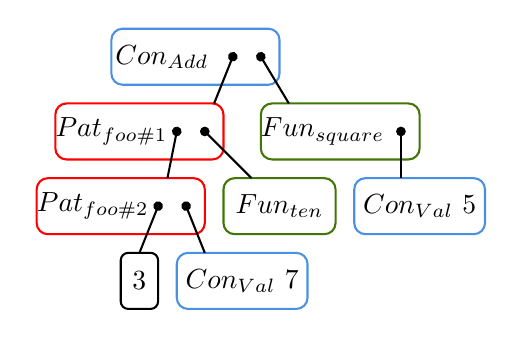
\begin{tikzpicture}[x=0.75pt,y=0.75pt,yscale=-0.9,xscale=0.9]
%uncomment if require: \path (0,440.8571319580078); %set diagram left start at 0, and has height of 440.8571319580078

%Rounded Rect [id:dp48618213158536694]
\draw  [color={rgb, 255:red, 74; green, 144; blue, 226 }  ,draw opacity=1 ] (190,196) .. controls (190,192.69) and (192.69,190) .. (196,190) -- (254,190) .. controls (257.31,190) and (260,192.69) .. (260,196) -- (260,214) .. controls (260,217.31) and (257.31,220) .. (254,220) -- (196,220) .. controls (192.69,220) and (190,217.31) .. (190,214) -- cycle ;

%Rounded Rect [id:dp009025103452140248]
\draw  [color={rgb, 255:red, 74; green, 144; blue, 226 }  ,draw opacity=1 ] (95,236) .. controls (95,232.69) and (97.69,230) .. (101,230) -- (159,230) .. controls (162.31,230) and (165,232.69) .. (165,236) -- (165,254) .. controls (165,257.31) and (162.31,260) .. (159,260) -- (101,260) .. controls (97.69,260) and (95,257.31) .. (95,254) -- cycle ;

%Rounded Rect [id:dp9232511876637792]
\draw  [color={rgb, 255:red, 74; green, 144; blue, 226 }  ,draw opacity=1 ] (60,116) .. controls (60,112.69) and (62.69,110) .. (66,110) -- (144,110) .. controls (147.31,110) and (150,112.69) .. (150,116) -- (150,134) .. controls (150,137.31) and (147.31,140) .. (144,140) -- (66,140) .. controls (62.69,140) and (60,137.31) .. (60,134) -- cycle ;

%Rounded Rect [id:dp10823094494105145]
\draw  [color={rgb, 255:red, 255; green, 0; blue, 0 }  ,draw opacity=1 ] (30,156) .. controls (30,152.69) and (32.69,150) .. (36,150) -- (114,150) .. controls (117.31,150) and (120,152.69) .. (120,156) -- (120,174) .. controls (120,177.31) and (117.31,180) .. (114,180) -- (36,180) .. controls (32.69,180) and (30,177.31) .. (30,174) -- cycle ;

%Rounded Rect [id:dp509725264431323]
\draw  [color={rgb, 255:red, 255; green, 0; blue, 0 }  ,draw opacity=1 ] (20,196) .. controls (20,192.69) and (22.69,190) .. (26,190) -- (104,190) .. controls (107.31,190) and (110,192.69) .. (110,196) -- (110,214) .. controls (110,217.31) and (107.31,220) .. (104,220) -- (26,220) .. controls (22.69,220) and (20,217.31) .. (20,214) -- cycle ;

%Rounded Rect [id:dp3455746100780601]
\draw   (65,234) .. controls (65,231.79) and (66.79,230) .. (69,230) -- (81,230) .. controls (83.21,230) and (85,231.79) .. (85,234) -- (85,256) .. controls (85,258.21) and (83.21,260) .. (81,260) -- (69,260) .. controls (66.79,260) and (65,258.21) .. (65,256) -- cycle ;

%Rounded Rect [id:dp5622973663481885]
\draw  [color={rgb, 255:red, 65; green, 117; blue, 5 }  ,draw opacity=1 ] (140,156) .. controls (140,152.69) and (142.69,150) .. (146,150) -- (219,150) .. controls (222.31,150) and (225,152.69) .. (225,156) -- (225,174) .. controls (225,177.31) and (222.31,180) .. (219,180) -- (146,180) .. controls (142.69,180) and (140,177.31) .. (140,174) -- cycle ;

%Rounded Rect [id:dp33414100410678915]
\draw  [color={rgb, 255:red, 65; green, 117; blue, 5 }  ,draw opacity=1 ] (120,196) .. controls (120,192.69) and (122.69,190) .. (126,190) -- (174,190) .. controls (177.31,190) and (180,192.69) .. (180,196) -- (180,214) .. controls (180,217.31) and (177.31,220) .. (174,220) -- (126,220) .. controls (122.69,220) and (120,217.31) .. (120,214) -- cycle ;

%Straight Lines [id:da7735002123972574]
\draw    (140,125) -- (155,150) ;

\draw [shift={(140,125)}, rotate = 59.04] [color={rgb, 255:red, 0; green, 0; blue, 0 }  ][fill={rgb, 255:red, 0; green, 0; blue, 0 }  ][line width=0.75]      (0, 0) circle [x radius= 2, y radius= 2]   ;
%Straight Lines [id:da19830589256441322]
\draw    (125,125) -- (115,150) ;

\draw [shift={(125,125)}, rotate = 111.8] [color={rgb, 255:red, 0; green, 0; blue, 0 }  ][fill={rgb, 255:red, 0; green, 0; blue, 0 }  ][line width=0.75]      (0, 0) circle [x radius= 2, y radius= 2]   ;
%Straight Lines [id:da7234273703208924]
\draw    (95,165) -- (90,190) ;

\draw [shift={(95,165)}, rotate = 101.31] [color={rgb, 255:red, 0; green, 0; blue, 0 }  ][fill={rgb, 255:red, 0; green, 0; blue, 0 }  ][line width=0.75]      (0, 0) circle [x radius= 2, y radius= 2]   ;
%Straight Lines [id:da39520289035501]
\draw    (110,165) -- (135,190) ;

\draw [shift={(110,165)}, rotate = 45] [color={rgb, 255:red, 0; green, 0; blue, 0 }  ][fill={rgb, 255:red, 0; green, 0; blue, 0 }  ][line width=0.75]      (0, 0) circle [x radius= 2, y radius= 2]   ;
%Straight Lines [id:da4431461097782077]
\draw    (215,165) -- (215,190) ;

\draw [shift={(215,165)}, rotate = 90] [color={rgb, 255:red, 0; green, 0; blue, 0 }  ][fill={rgb, 255:red, 0; green, 0; blue, 0 }  ][line width=0.75]      (0, 0) circle [x radius= 2, y radius= 2]   ;
%Straight Lines [id:da8121818084178258]
\draw    (85,205) -- (75,230) ;

\draw [shift={(85,205)}, rotate = 111.8] [color={rgb, 255:red, 0; green, 0; blue, 0 }  ][fill={rgb, 255:red, 0; green, 0; blue, 0 }  ][line width=0.75]      (0, 0) circle [x radius= 2, y radius= 2]   ;
%Straight Lines [id:da8679389234287274]
\draw    (100,205) -- (110,230) ;

\draw [shift={(100,205)}, rotate = 68.2] [color={rgb, 255:red, 0; green, 0; blue, 0 }  ][fill={rgb, 255:red, 0; green, 0; blue, 0 }  ][line width=0.75]      (0, 0) circle [x radius= 2, y radius= 2]   ;

% Text Node
\draw (225,205) node   {$Con_{Val} \ 5$};
% Text Node
\draw (130,245) node   {$Con_{Val} \ 7$};
% Text Node
\draw (87,125) node   {$Con_{Add}$};
% Text Node
\draw (60,165) node   {$Pat_{foo\#1}$};
% Text Node
\draw (50,205) node   {$Pat_{foo\#2}$};
% Text Node
\draw (75,245) node   {$3$};
% Text Node
\draw (173.05,165) node   {$Fun_{square}$};
% Text Node
\draw (150,205) node   {$Fun_{ten}$};

\end{tikzpicture}

% %   \caption{Some caption.}
% %   \label{fig:val}
% % \end{figure}


% We want to remark that, for space reasons, we were only able to introduce the
% representation of a rather simple target data type.
% %
% In practice, this reasoning can be extended to mutually recursive and parametric
% types as well.


% Overall, this approach offers significant advantages over the usual type-driven
% derivation of random generators:
% %
% \begin{itemize}
% \item \textbf{Composability:} we can combine different atomic representations
%   using different structure information sources depending on what property or
%   sub-system we need to verify using randomly generated values.
%   %
% \item \textbf{Extensibility:} the developer can derive representations for new
%   sources of structure information and combine them with the existing ones
%   simply by adding them to the existing generation specification of the target
%   data type.
%   %
% \item \textbf{Predictability:} using branching processes theory, it is possible
%   to predict the average distribution of generated values in terms of number of
%   constructors.
%   %
%   This prediction is completely modular, and can be obtained for any composite
%   representation obtained using the automatically derived |HRep|s and the
%   provided combinators.
% \end{itemize}

% \todo[author=AM, inline]{Maybe we can show an example random value from the representation
%   and its corresponding target value }



% \begin{align*}
%   \llbracket \_ \rrbracket_{target}\ :\ rep_{target}\ \rightarrow\ target
% \end{align*}
%
% \begin{code}
% class (rep down target) where
%   step :: rep target -> target
% \end{code}
%
% \begin{code}
% data (Term f) a = TagTerm (f a)

% \begin{code}
% instance (HRep_Val down Exp) where
%   step (Mk_Val n) = Val n

% instance (HRep_Add down Exp) where
%   step (Mk_Add x y) = Add x y

% instance (HRep_Mul down Exp) where
%   step (Mk_Mul x y) = Mul x y
% \end{code}

% \begin{code}
% instance (f otimes n down Exp) where
%   step (Freq f) = step f
% \end{code}

% \begin{code}
% instance Arbitrary1 (f otimes n) where
%   liftArbitrary gen_HRep = Tag <$> gen_HRep
% \end{code} %$

% instance (Term f down Exp) where
%   step (TagTerm f) = step f
% \end{code}

% \begin{code}
% instance (HRep_ten down Exp) where
%   step Mk_ten = ten

% instance (HRep_square down Exp) where
%   step (Mk_square x) = square x

% instance (HRep_minus down Exp) where
%   step (Mk_minus x y) = minus x y
% \end{code}

% \begin{code}
% instance Arbitrary1 HRep_ten where
%   liftArbitrary gen_HRep = pure Mk_ten

% instance Arbitrary1 HRep_square where
%   liftArbitrary gen_HRep = Mk_square <$> gen_HRep

% instance Arbitrary1 HRep_minus where
%   liftArbitrary gen_HRep
%     = Mk_minus <$> gen_HRep <*> gen_HRep
% \end{code} %$

% \begin{code}
% instance (HRep_foo_1 down Exp) where
%   step (Mk_foo_1 x y)
%     = Add (Add x (Val 50)) (Add (Val 25) y)

% instance (HRep_foo_2 down Exp) where
%   step (Mk_foo_2 x y)
%     = Mul (Val 50) (Mul (Val x) y)
% \end{code}

% \begin{code}
% instance Arbitrary1 HRep_foo_1 where
%   liftArbitrary gen_HRep
%     = Mk_foo_1 <$> gen_HRep <*> gen_HRep

% instance Arbitrary1 HRep_foo_2 where
%   liftArbitrary gen_HRep
%     = Mk_foo_2 <$> arbitrary <*> gen_HRep
% \end{code} %$

% \begin{code}
% instance (f oplus g down Exp) where
%   step (L f) = step f
%   step (R g) = step g
% \end{code}

% \begin{code}
% instance Arbitrary1 (f oplus g) where
%   liftArbitrary gen_HRep
%     = frequency
%       [ (freq at_f, L <$> gen_HRep)
%       , (freq at_g, R <$> gen_HRep) ]
% \end{code} %$

% \begin{figure}[b]
%   \centering
%   
\tikzset{every picture/.style={line width=0.75pt}} %set default line width to 0.75pt

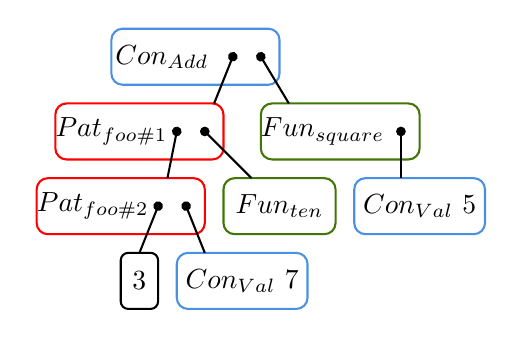
\begin{tikzpicture}[x=0.75pt,y=0.75pt,yscale=-0.9,xscale=0.9]
%uncomment if require: \path (0,440.8571319580078); %set diagram left start at 0, and has height of 440.8571319580078

%Rounded Rect [id:dp48618213158536694]
\draw  [color={rgb, 255:red, 74; green, 144; blue, 226 }  ,draw opacity=1 ] (190,196) .. controls (190,192.69) and (192.69,190) .. (196,190) -- (254,190) .. controls (257.31,190) and (260,192.69) .. (260,196) -- (260,214) .. controls (260,217.31) and (257.31,220) .. (254,220) -- (196,220) .. controls (192.69,220) and (190,217.31) .. (190,214) -- cycle ;

%Rounded Rect [id:dp009025103452140248]
\draw  [color={rgb, 255:red, 74; green, 144; blue, 226 }  ,draw opacity=1 ] (95,236) .. controls (95,232.69) and (97.69,230) .. (101,230) -- (159,230) .. controls (162.31,230) and (165,232.69) .. (165,236) -- (165,254) .. controls (165,257.31) and (162.31,260) .. (159,260) -- (101,260) .. controls (97.69,260) and (95,257.31) .. (95,254) -- cycle ;

%Rounded Rect [id:dp9232511876637792]
\draw  [color={rgb, 255:red, 74; green, 144; blue, 226 }  ,draw opacity=1 ] (60,116) .. controls (60,112.69) and (62.69,110) .. (66,110) -- (144,110) .. controls (147.31,110) and (150,112.69) .. (150,116) -- (150,134) .. controls (150,137.31) and (147.31,140) .. (144,140) -- (66,140) .. controls (62.69,140) and (60,137.31) .. (60,134) -- cycle ;

%Rounded Rect [id:dp10823094494105145]
\draw  [color={rgb, 255:red, 255; green, 0; blue, 0 }  ,draw opacity=1 ] (30,156) .. controls (30,152.69) and (32.69,150) .. (36,150) -- (114,150) .. controls (117.31,150) and (120,152.69) .. (120,156) -- (120,174) .. controls (120,177.31) and (117.31,180) .. (114,180) -- (36,180) .. controls (32.69,180) and (30,177.31) .. (30,174) -- cycle ;

%Rounded Rect [id:dp509725264431323]
\draw  [color={rgb, 255:red, 255; green, 0; blue, 0 }  ,draw opacity=1 ] (20,196) .. controls (20,192.69) and (22.69,190) .. (26,190) -- (104,190) .. controls (107.31,190) and (110,192.69) .. (110,196) -- (110,214) .. controls (110,217.31) and (107.31,220) .. (104,220) -- (26,220) .. controls (22.69,220) and (20,217.31) .. (20,214) -- cycle ;

%Rounded Rect [id:dp3455746100780601]
\draw   (65,234) .. controls (65,231.79) and (66.79,230) .. (69,230) -- (81,230) .. controls (83.21,230) and (85,231.79) .. (85,234) -- (85,256) .. controls (85,258.21) and (83.21,260) .. (81,260) -- (69,260) .. controls (66.79,260) and (65,258.21) .. (65,256) -- cycle ;

%Rounded Rect [id:dp5622973663481885]
\draw  [color={rgb, 255:red, 65; green, 117; blue, 5 }  ,draw opacity=1 ] (140,156) .. controls (140,152.69) and (142.69,150) .. (146,150) -- (219,150) .. controls (222.31,150) and (225,152.69) .. (225,156) -- (225,174) .. controls (225,177.31) and (222.31,180) .. (219,180) -- (146,180) .. controls (142.69,180) and (140,177.31) .. (140,174) -- cycle ;

%Rounded Rect [id:dp33414100410678915]
\draw  [color={rgb, 255:red, 65; green, 117; blue, 5 }  ,draw opacity=1 ] (120,196) .. controls (120,192.69) and (122.69,190) .. (126,190) -- (174,190) .. controls (177.31,190) and (180,192.69) .. (180,196) -- (180,214) .. controls (180,217.31) and (177.31,220) .. (174,220) -- (126,220) .. controls (122.69,220) and (120,217.31) .. (120,214) -- cycle ;

%Straight Lines [id:da7735002123972574]
\draw    (140,125) -- (155,150) ;

\draw [shift={(140,125)}, rotate = 59.04] [color={rgb, 255:red, 0; green, 0; blue, 0 }  ][fill={rgb, 255:red, 0; green, 0; blue, 0 }  ][line width=0.75]      (0, 0) circle [x radius= 2, y radius= 2]   ;
%Straight Lines [id:da19830589256441322]
\draw    (125,125) -- (115,150) ;

\draw [shift={(125,125)}, rotate = 111.8] [color={rgb, 255:red, 0; green, 0; blue, 0 }  ][fill={rgb, 255:red, 0; green, 0; blue, 0 }  ][line width=0.75]      (0, 0) circle [x radius= 2, y radius= 2]   ;
%Straight Lines [id:da7234273703208924]
\draw    (95,165) -- (90,190) ;

\draw [shift={(95,165)}, rotate = 101.31] [color={rgb, 255:red, 0; green, 0; blue, 0 }  ][fill={rgb, 255:red, 0; green, 0; blue, 0 }  ][line width=0.75]      (0, 0) circle [x radius= 2, y radius= 2]   ;
%Straight Lines [id:da39520289035501]
\draw    (110,165) -- (135,190) ;

\draw [shift={(110,165)}, rotate = 45] [color={rgb, 255:red, 0; green, 0; blue, 0 }  ][fill={rgb, 255:red, 0; green, 0; blue, 0 }  ][line width=0.75]      (0, 0) circle [x radius= 2, y radius= 2]   ;
%Straight Lines [id:da4431461097782077]
\draw    (215,165) -- (215,190) ;

\draw [shift={(215,165)}, rotate = 90] [color={rgb, 255:red, 0; green, 0; blue, 0 }  ][fill={rgb, 255:red, 0; green, 0; blue, 0 }  ][line width=0.75]      (0, 0) circle [x radius= 2, y radius= 2]   ;
%Straight Lines [id:da8121818084178258]
\draw    (85,205) -- (75,230) ;

\draw [shift={(85,205)}, rotate = 111.8] [color={rgb, 255:red, 0; green, 0; blue, 0 }  ][fill={rgb, 255:red, 0; green, 0; blue, 0 }  ][line width=0.75]      (0, 0) circle [x radius= 2, y radius= 2]   ;
%Straight Lines [id:da8679389234287274]
\draw    (100,205) -- (110,230) ;

\draw [shift={(100,205)}, rotate = 68.2] [color={rgb, 255:red, 0; green, 0; blue, 0 }  ][fill={rgb, 255:red, 0; green, 0; blue, 0 }  ][line width=0.75]      (0, 0) circle [x radius= 2, y radius= 2]   ;

% Text Node
\draw (225,205) node   {$Con_{Val} \ 5$};
% Text Node
\draw (130,245) node   {$Con_{Val} \ 7$};
% Text Node
\draw (87,125) node   {$Con_{Add}$};
% Text Node
\draw (60,165) node   {$Pat_{foo\#1}$};
% Text Node
\draw (50,205) node   {$Pat_{foo\#2}$};
% Text Node
\draw (75,245) node   {$3$};
% Text Node
\draw (173.05,165) node   {$Fun_{square}$};
% Text Node
\draw (150,205) node   {$Fun_{ten}$};

\end{tikzpicture}

%   \caption{Higher level representation of the data type |Exp|, defined using
%     structural information from the function |foo| and the abstract interface of
%     the module |M|.}
%   \label{fig:hrep}
% \end{figure}


% Local Variables:
% TeX-master: "main.lhs.tex"
% TeX-command-default: "Make"
% End:
